% Plantilla para documentos LaTeX para enunciados
% Por Pedro Pablo Aste Kompen - ppaste@uc.cl
% Licencia Creative Commons BY-NC-SA 3.0
% http://creativecommons.org/licenses/by-nc-sa/3.0/

\documentclass[12pt]{article}

% Margen de 1 pulgada por lado
\usepackage{fullpage}
% Incluye gráficas
\usepackage{graphicx}
% Packages para matemáticas, por la American Mathematical Society
\usepackage{amssymb}
\usepackage{amsmath}
% Desactivar hyphenation
\usepackage[none]{hyphenat}
% Saltar entre párrafos - sin sangrías
\usepackage{parskip}
% Español y UTF-8
\usepackage[spanish]{babel}
\usepackage[utf8]{inputenc}
% Links en el documento
\usepackage{hyperref}
\usepackage{fancyhdr}
\setlength{\headheight}{15.2pt}
\setlength{\headsep}{5pt}
\pagestyle{fancy}

\newcommand{\N}{\mathbb{N}}
\newcommand{\Exp}[1]{\mathcal{E}_{#1}}
\newcommand{\List}[1]{\mathcal{L}_{#1}}
\newcommand{\EN}{\Exp{\N}}
\newcommand{\LN}{\List{\N}}

\newcommand{\comment}[1]{}
\newcommand{\lb}{\\~\\}
\newcommand{\eop}{_{\square}}
\newcommand{\hsig}{\hat{\sigma}}
\newcommand{\ra}{\rightarrow}
\newcommand{\lra}{\leftrightarrow}

% Cambiar por nombre completo + número de alumno
\newcommand{\alumno}{Victor Ruiz - 2320012J}
\rhead{Tarea 1 - \alumno}

\begin{document}
\thispagestyle{empty}
% Membrete
% PUC-ING-DCC-IIC1103
\begin{minipage}{2.3cm}
\includegraphics[width=2cm]{img/logo.pdf}
\vspace{0.5cm} % Altura de la corona del logo, así el texto queda alineado verticalmente con el círculo del logo.
\end{minipage}
\begin{minipage}{\linewidth}
\textsc{\raggedright \footnotesize
Pontificia Universidad Católica de Chile \\
Departamento de Ciencia de la Computación \\
IIC2613 Inteligencia Artificial \\}
\end{minipage}


% Titulo
\begin{center}
\vspace{0.5cm}
{\huge\bf Tarea 1}\\
\vspace{0.2cm}
\today\\
\vspace{0.2cm}
\footnotesize{1º semestre 2025 -  Profesores Hans Lobel - Jorge Baier}\\
\vspace{0.2cm}
\footnotesize{\alumno}
\rule{\textwidth}{0.05mm}
\end{center}



\section*{Respuestas}

\subsection*{1. Trabajo a futuro}\subsubsection*{(a)}  

1. \textbf{Resiliencia}: Soy de esos que no se achican cuando todo se pone cuesta arriba. Si hay presión en el trabajo o un problema personal, me relajo, pienso fríamente y busco alternativas. Por ejemplo, en proyectos con plazos imposibles, no me estreso: reorganizo prioridades, aprendo de los errores y sigo adelante. ¿Un ejemplo? Remonte discretas en el Examen, siendo que necesitaba un 3.9 para pasar el ramo, saqué 4.0 y eso que el día anterior tuve Examen de Calculo 3.

2. \textbf{Toma de decisiones}: Tengo buen ojo para decidir rápido sin perder la cabeza. Analizo pros y contras, pero también confío en mi instinto. Una vez, en un equipo con conflicto por recursos, reasigné tareas en media hora (sin reuniones eternas) y todos quedaron contentos. Mis compañeros dicen que tengo 'don' para evitar la parálisis por análisis.  

3. \textbf{Liderazgo}: No soy de jefes autoritarios. Prefiero escuchar, dar libertad y sacar lo mejor de cada uno. Logramos sacar adelante el proyecto CPU Te Ayuda (proyecto que buscaba reacondicionar notebooks en desuso, para luego donarlos a estudiantes de ingenieria que necesitaran uno urgente) de la iniciativa CPU (fui coordi general durante todo el año pasado) porque delegué tareas según habilidades y motivaciones. Y cuando hubo problemas, no culpé a nadie, sino que propuse soluciones en conjunto.

\subsubsection*{(b)}  

\textbf{Actividades que generan ``Flow'' en mi experiencia:}  

1. \textbf{Entrenamiento de fuerza con pesas}: Cuando levanto hierros, el mundo desaparece. Me fijo metas simples: 'hoy hago 2 repes más' o 'perfecciono la técnica'. Siento cada músculo, ajusto la respiración y me vuelvo una máquina. Si subo de peso, celebro; si fallo, anoto qué mejorar. Es mi terapia antiestrés. En mi último ciclo de entrenamiento, me propuse hacer 10 dominadas perfectas. Tras semanas ajustando agarres y midiendo descansos, lo logré. La concentración en cada movimiento me hacía perder la noción del tiempo, y el progreso semanal reforzaba la motivación.  

2. \textbf{Cocinar}: Cocinar es como un laberinto creativo. A veces sigo recetas al pie de la letra; otras, invento con lo que hay en la refri. Concentrarme en no quemar la salsa, equilibrar sabores y que quede bonito me hace olvidar el celular. Y cuando alguien prueba el plato y dice 'te queo weno', siento que gané MasterChef. Preparé ramen desde cero. Fue un desafío de 3 horas, pero cada paso (caldo, fideos, toppings) era un logro en sí mismo. 
Al final, ver el plato colorido y sabroso me daba una satisfacción inigualable.  

3. \textbf{Planificación estratégica en Google Calendar}: Soy adicto a organizar mi semana. Bloqueo horas para trabajar, hacer ejercicio y hasta para no hacer nada. Ver todo en colores me da paz mental. Si algo se desordena, lo reajusto sin drama. Y tachar tareas completadas es como ganar niveles en un videojuego. Durante los exámenes del semestre pasado, organicé 72 horas de estudio en bloques de 90 minutos (técnica Pomodoro extendida). Usé etiquetas para temas prioritarios y ajustes dinámicos cuando un ejercicio me tomaba más de lo previsto. Al final, logré pasar Discretas y Calculo 3.
\subsubsection*{(c)}

\textbf{Tres problemáticas globales donde podría contribuir}:
\begin{itemize}
    \item \textbf{Optimización sostenible de cadenas de suministro}: Para enfrentar interrupciones (ej.: pandemias o desastres naturales), mi resiliencia permite adaptar estrategias rápidamente (como rediseñar rutas logísticas). Mi toma de decisiones ágil prioriza criterios de sostenibilidad (reducir huella de carbono) sin sacrificar eficiencia, incluso bajo incertidumbre.
    \item \textbf{Mitigación de sesgos algorítmicos en sistemas de IA}: Mi capacidad para analizar datos críticamente (ej.: identificar variables proxy discriminatorias como el código postal) y decidir entre precisión vs. equidad es clave. Además, mi liderazgo inclusivo fomenta equipos multidisciplinarios (éticos, ingenieros, legisladores) para diseñar soluciones justas y escalables.
    \item \textbf{Digitalización inclusiva de servicios públicos}: Liderar proyectos que integren tecnología en comunidades marginadas (ej.: apps de salud en zonas rurales sin internet) requiere coordinar gobiernos, ONGs y usuarios. Mi resiliencia ayuda a superar barreras como la resistencia al cambio o fallos técnicos recurrentes, manteniendo el enfoque en el impacto social a largo plazo.
\end{itemize}

\textbf{Mitigación de sesgos algorítmicos en sistemas de IA}: Los sesgos algorítmicos son distorsiones sistemáticas en los resultados de modelos de inteligencia artificial que replican o amplifican prejuicios sociales, afectando decisiones críticas en áreas como contrataciones laborales, préstamos bancarios, justicia penal o acceso a servicios públicos. Estos sesgos surgen de múltiples factores: datos históricos contaminados con discriminación estructural (ej.: registros policiales que sobre representan a minorías étnicas), diseños de modelos que priorizan la eficiencia sobre la equidad, y equipos de desarrollo con poca diversidad sociocultural. Un ejemplo emblemático es el estudio de Buolamwini y Gebru (2018), que demostró que los sistemas de reconocimiento facial comerciales tenían tasas de error hasta un 34\% mayores para rostros de mujeres de piel oscura, comparado con hombres blancos. Paralelamente, algoritmos utilizados en evaluaciones de crédito han mostrado discriminación indirecta hacia grupos marginados, como mujeres o comunidades étnicas, al basarse en variables proxy como el código postal o historiales laborales truncados por brechas de género (O’Neil, 2016).

La relevancia de esta problemática radica en su impacto transversal, que trasciende lo técnico para infiltrarse en lo social, económico y político. En primer lugar, perpetúa injusticias estructurales al automatizar la exclusión. Por ejemplo, sistemas de selección laboral que descartan currículos de personas con nombres asociados a minorías, o herramientas predictivas policiales que etiquetan barrios racializados como «de alto riesgo», reforzando ciclos de vigilancia excesiva. Esto no solo limita oportunidades individuales, sino que cristaliza desigual-\\-dades a escala sistémica. En segundo término, la opacidad de muchos algoritmos erosiona la confianza pública en instituciones clave. Cuando un ciudadano no comprende por qué se le denegó un préstamo o una libertad condicional, surge desconfianza hacia bancos o sistemas judiciales, como advierte Crawford (2021) en su análisis sobre la IA como herramienta de poder asimétrico. Finalmente, los riesgos legales y financieros son inevitables: empresas como Amazon tuvieron que retirar algoritmos de contratación tras descubrir sesgos contra mujeres, mientras que el sistema COMPAS, utilizado en tribunales estadounidenses para predecir reincidencia, demostró discriminar a afroamericanos, generando demandas multimillonarias y daños reputacionales (ProPublica, 2016).

Esta problemática se agrava con la escalada de la IA en sectores sensibles. Sin mecanismos robustos de auditoría ética y participación diversa en el desarrollo tecnológico, los sesgos algorítmicos no son un error técnico, sino una amenaza para la justicia social y la estabilidad institucional. Como señala Barocas et al. (2019), la solución requiere integrar enfoques interdisciplinarios: desde técnicas de machine learning justo hasta marcos legales que exijan transparencia algorítmica.

\textbf{Contribución con mis habilidades y formación}:
\begin{itemize}
    \item \textbf{Resiliencia}: Desarrollar modelos libres de sesgos requiere iteración constante ante datos incompletos o contextos cambiantes. Por ejemplo, ajustar algoritmos para adaptarse a nuevas normativas éticas (ej.: regulaciones de la UE sobre IA) implica persistencia en pruebas técnicas y negociaciones con stakeholders.
    \item \textbf{Toma de decisiones}: Priorizar métricas de equidad (ej.: paridad demográfica en resultados) frente a la eficiencia pura (ej.: precisión del modelo). Esto implica análisis costo-beneficio riguroso, usando herramientas como fairness-aware machine learning (Barocas et al., 2019).
    \item \textbf{Liderazgo}: Coordinar equipos multidisciplinarios (ingenieros, científicos sociales, abogados) para integrar perspectivas diversas en el diseño de sistemas. Por ejemplo, liderar workshops de ética algorítmica en organizaciones, asegurando que las soluciones técnicas se alineen con valores humanos. 
\end{itemize}

\textbf{Conexión con el estado de flow}:
\begin{itemize}
    \item \textbf{Desafío vs. habilidad equilibrados}: La complejidad técnica de ajustar modelos (ej.: implementar técnicas de debiasing) exige un dominio avanzado de IA, alineado con mi formación.
    \item \textbf{Metas claras y feedback inmediato}: Cada iteración del modelo ofrece datos concretos (ej.: reducción de disparidades en métricas de equidad), permitiendo ajustes iterativos.
    \item \textbf{Concentración absoluta}: Actividades como depurar código, analizar matrices de confusión o diseñar interfaces explicativas (XAI) demandan enfoque prolongado, eliminando distracciones. 
\end{itemize}

\subsubsection*{(d)}

\begin{figure}[h]
    \centering
    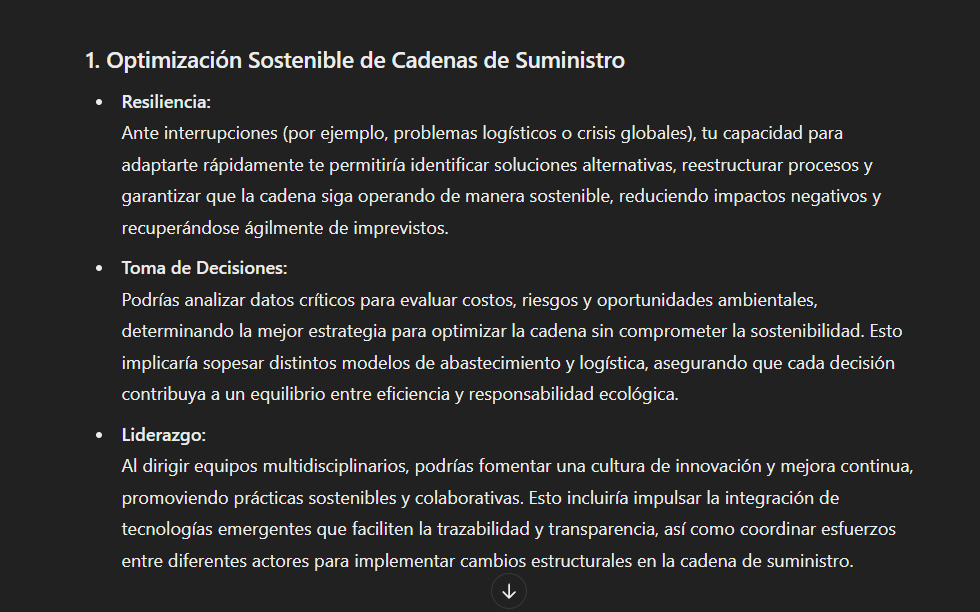
\includegraphics[width=0.9\textwidth]{img/problematica_1.png}
    \caption{Como aplicar mis habilidades en la primera problematica segun ChatGPT}
\end{figure}

\begin{figure}[h]
    \centering
    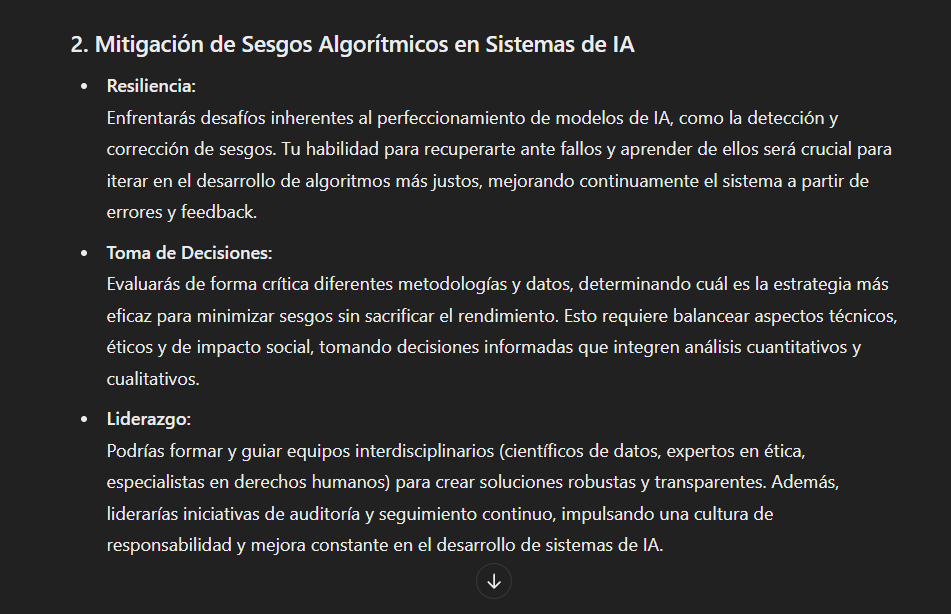
\includegraphics[width=0.9\textwidth]{img/problematica_2.png}
    \caption{Como aplicar mis habilidades en la segunda problematica segun ChatGPT}
\end{figure}
\begin{figure}[h]
    \centering
    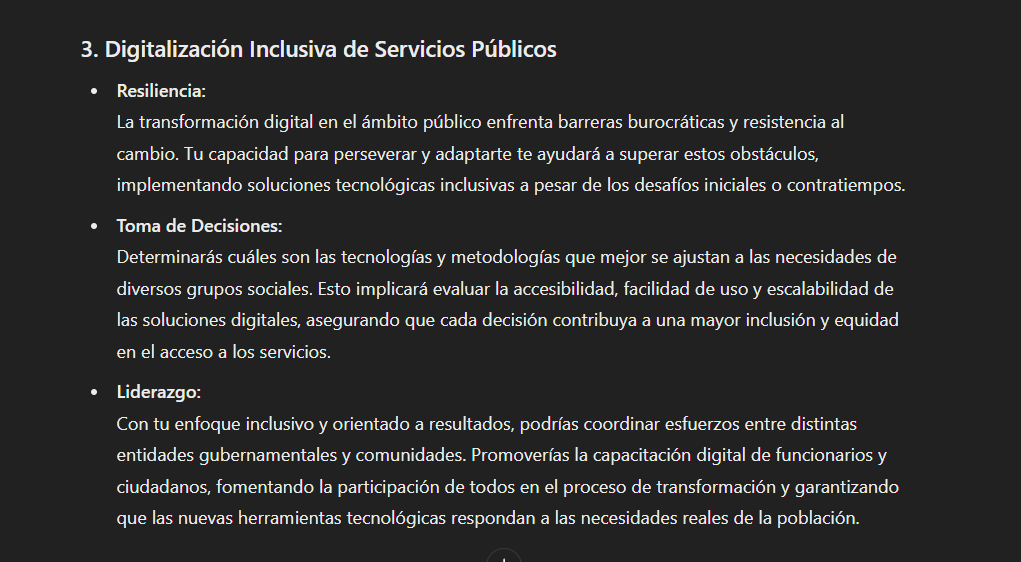
\includegraphics[width=0.9\textwidth]{img/problematica_3.png}
    \caption{Como aplicar mis habilidades en la tercera problematica segun ChatGPT}
\end{figure}
\clearpage

\subsubsection*{(e)}

\textbf{Evaluación crítica a la respuesta de ChatGPT:}  

La respuesta inicial acierta en vincular habilidades con problemáticas de forma general (ej.: resiliencia en cadenas de suministro), pero carece de propuestas concretas. Para mejorarla, sugiero:  

\begin{itemize}  
    \item \textbf{Optimización de cadenas de suministro}:  
    - Incluir metodologías como \textit{Lean Six Sigma} \cite{LeanSixSigma} y herramientas como \textit{AnyLogic} \cite{AnyLogic} para simular escenarios.  
    - Ejemplos específicos: uso de algoritmos de enrutamiento (\textit{Vehicle Routing Problem} \cite{VehicleRouting}) o blockchain \cite{BlockchainIBM} para trazabilidad.  
    - Definir KPIs medibles (ej.: reducir emisiones en 20\% \cite{LeanSixSigma}).  

    \item \textbf{Mitigación de sesgos en IA}:  
    - Añadir técnicas como \textit{adversarial debiasing} \cite{AdversarialDebiasing} y frameworks como \textit{Fairlearn} \cite{Fairlearn} para cuantificar sesgos.  
    - Propuestas prácticas: talleres de \textit{Design Thinking} \cite{DesignThinking} para alinear equipos y pruebas A/B con comunidades afectadas \cite{CommunityHackathons}.  
    - Implementar transparencia mediante informes públicos de impacto \cite{Barocas2019}.  

    \item \textbf{Digitalización inclusiva}:  
    - Establecer estándares técnicos (ej.: WCAG 2.1 \cite{WCAG21}) y soluciones \textit{offline-first} \cite{OfflineFirst}.  
    - Métricas claras: aumentar acceso a salud en 40\% \cite{CommunityHackathons} en zonas rurales.  
    - Mecanismos participativos: hackatones comunitarios \cite{CommunityHackathons} y mesas de trabajo con líderes locales \cite{DesignThinking}.  
\end{itemize} 

\subsection*{2. Rol de la Inteligencia Artificial en tu futuro}

\subsubsection*{(a)}

La inteligencia artificial (IA) desempeña un rol dual en esta problemática: es tanto fuente del problema como herramienta clave para su solución. Por un lado, los sistemas de IA heredan y amplifican sesgos sociales al entrenarse con datos históricos que reflejan discriminación estructural. Por ejemplo, algoritmos de reclutamiento laboral entrenados con currículos de décadas pasadas (donde hombres blancos dominaban ciertas industrias) replican esos patrones, excluyendo a mujeres o minorías étnicas (O’Neil, 2016). Del mismo modo, modelos predictivos en justicia penal, como COMPAS, perpetúan desigualdades raciales al basarse en datos policiales sesgados (ProPublica, 2016).

Sin embargo, la IA también ofrece métodos innovadores para detectar, cuantificar y corregir estos sesgos. Técnicas como fairness-aware machine learning permiten integrar métricas de equidad (ej.: paridad demográfica, igualdad de oportunidades) en el entrenamiento de modelos. Por ejemplo, el reequilibrio de datasets mediante oversampling de grupos subrepresentados o el uso de algoritmos de debiasing (como adversarial learning) ajustan las predicciones para minimizar disparidades (Barocas et al., 2019). Además, herramientas de explicabilidad (XAI) hacen transparente la lógica interna de los modelos, identificando variables proxy discriminatorias (ej.: código postal como sustituto de etnia).

El desafío radica en que la IA no es neutral: su capacidad para mitigar sesgos depende de diseños intencionales éticos y diversidad en los equipos de desarrollo. Aquí es donde habilidades como el liderazgo inclusivo y la toma de decisiones basada en evidencia son críticas. Por ejemplo, liderar proyectos que integren a científicos de datos con especialistas en ética y comunidades afectadas asegura que los modelos no solo sean técnicamente robustos, sino socialmente responsables. Asimismo, la resiliencia es clave para iterar modelos ante nuevos sesgos emergentes, como los derivados de cambios legislativos o dinámicas sociales.

En síntesis, la IA es un arma de doble filo: sin regulación y enfoque ético, profundiza desigualdades; con gobernanza adecuada y técnicas avanzadas, se convierte en un motor de equidad. Su rol, por tanto, no es autónomo, sino mediado por la intencionalidad humana y los marcos éticos que la guían.

\subsubsection*{(b)}

1. \textbf{Planificación y Búsqueda Heurística}: \textbf{NO se relaciona.} Esta área se enfoca en diseñar estrategias para alcanzar metas mediante secuencias de acciones (ej.: resolver laberintos, optimizar rutas). La mitigación de sesgos no requiere planificación de pasos físicos o lógicos para alcanzar un objetivo, sino técnicas específicas de análisis de datos y ajuste de modelos, fuera del ámbito de la búsqueda heurística.

2. \textbf{Representación Lógica del Conocimiento y Razonamiento}: \textbf{SÍ se relaciona.} La representación lógica permite formalizar reglas éticas y restricciones para evitar sesgos. Por ejemplo, definir axiomas como "un algoritmo de contratación no debe considerar género" y usar razonamiento deductivo para verificar su cumplimiento. Además, sistemas como Clingo (ASP) pueden modelar escenarios para detectar inconsistencias en datos o decisiones algorítmicas.

3. \textbf{Procesamiento de Lenguaje Natural (PLN)}: \textbf{SÍ se relaciona.} Los sesgos en modelos de lenguaje (ej.: asociar "enfermera" con mujeres o "director" con hombres) son un subproblema crítico. Mitigar estos sesgos implica ajustar embeddings, eliminar estereotipos en corpus de entrenamiento y aplicar técnicas de debiasing específicas para PLN, como métodos de contraste contextual.

4. \textbf{Visión por Computador}: \textbf{SÍ se relaciona.} Los sesgos en reconocimiento facial (ej.: menor precisión para rostros de piel oscura) son un problema documentado. Corregirlos requiere rebalancear datasets, aplicar aumentos de datos específicos y evaluar métricas de equidad en modelos de visión, áreas directamente vinculadas a esta disciplina.

5. \textbf{Aprendizaje automático}: \textbf{SÍ se relaciona.} Es el núcleo técnico de la mitigación de sesgos. Técnicas como fairness-aware machine learning, algoritmos de reequilibrio de datos (oversampling), y métricas de equidad (paridad demográfica, igualdad de oportunidades) pertenecen a esta área. Además, métodos de explicabilidad (XAI) ayudan a identificar fuentes de sesgo en modelos predictivos.


\subsubsection*{(c)}  

La solución de la problemática de mitigación de sesgos algorítmicos \textbf{requiere principalmente el Sistema 2}, pero con un apoyo secundario del Sistema 1. El Sistema 1, responsable de procesos automáticos e intuitivos (como reconocer patrones superficiales de exclusión en un modelo de contratación), puede ser útil en etapas iniciales para identificar anomalías evidentes. Por ejemplo, un experto podría notar rápidamente que un algoritmo ignora a un grupo demográfico, activando una alerta inicial. Sin embargo, esta capacidad intuitiva es insuficiente para abordar sesgos estructurales, como correlaciones ocultas entre variables (ej.: código postal vinculado a etnia), que requieren un análisis metódico y consciente.  

El Sistema 2, en cambio, es indispensable para desentrañar la complejidad técnica y ética del problema. Su rol se manifiesta en tres acciones críticas:  

1. \textbf{Análisis riguroso de datos}: Evaluar distribuciones demográficas y aplicar métricas de equidad (paridad estadística, igualdad de oportunidades), lo que exige atención sostenida y uso de herramientas como *fairness-aware machine learning*.  

2. \textbf{Diseño ético de modelos}: Implementar reglas lógicas que excluyan variables discriminatorias, utilizando sistemas como ASP/Clingo para formalizar restricciones (ej.: "no usar género en decisiones de crédito").  

3. \textbf{Validación iterativa}: Realizar pruebas estadísticas y ciclos de retroalimentación con grupos afectados, procesos que demandan adaptación constante y evaluación crítica de resultados.  

Aunque el Sistema 1 puede acelerar la detección inicial de sesgos, su naturaleza superficial y rápida no permite corregir problemas arraigados en datos o lógicas algorítmicas. Por ello, el Sistema 2 domina la solución, mientras que el Sistema 1 actúa como un complemento limitado pero no prescindible. En síntesis, ambos sistemas colaboran, pero el peso recae en el razonamiento consciente y estructurado del Sistema 2 para garantizar soluciones justas y sostenibles.  

\newpage

\begin{thebibliography}{9}

\bibitem{buolamwini2018} 
Buolamwini, J., \& Gebru, T. (2018). Gender Shades: Intersectional Accuracy Disparities in Commercial Gender Classification. *Proceedings of Machine Learning Research*, 81, 1-15. Recuperado desde \url{http://proceedings.mlr.press/v81/buolamwini18a.html}

\bibitem{ONeil2016} 
O’Neil, C. (2016). *Weapons of Math Destruction: How Big Data Increases Inequality and Threatens Democracy*. Crown Publishing Group.

\bibitem{Crawford2021} 
Crawford, K. (2021). *Atlas of AI: Power, Politics, and the Planetary Costs of Artificial Intelligence*. Yale University Press.

\bibitem{ProPublica2016} 
ProPublica. (2016). Machine Bias. Recuperado desde \url{https://www.propublica.org/article/machine-bias-risk-assessments-in-criminal-sentencing}

\bibitem{Barocas2019} 
Barocas, S., Hardt, M., \& Narayanan, A. (2019). *Fairness and Machine Learning*. Recuperado desde \url{https://fairmlbook.org}

\bibitem{LeanSixSigma} 
Motorola University. (2023). \textit{What is Lean Six Sigma?} Recuperado desde \url{https://www.motorolauniversity.com}

\bibitem{AnyLogic} 
AnyLogic. (2023). \textit{Simulation Software for Supply Chain Optimization}. Recuperado desde \url{https://www.anylogic.com}

\bibitem{VehicleRouting} 
Toth, P., \& Vigo, D. (2014). \textit{Vehicle Routing: Problems, Methods, and Applications}. SIAM.

\bibitem{BlockchainIBM} 
IBM. (2023). \textit{Blockchain for Supply Chain Transparency}. Recuperado desde \url{https://www.ibm.com/blockchain/supply-chain}

\bibitem{Fairlearn} 
Bird, S. et al. (2020). \textit{Fairlearn: A Toolkit for Assessing and Improving Fairness in AI}. Microsoft Research. Recuperado desde \url{https://fairlearn.org}

\bibitem{AdversarialDebiasing} 
Zhang, B. H. et al. (2018). \textit{Mitigating Unwanted Biases with Adversarial Learning}. Proceedings of AIES.

\bibitem{WCAG21} 
W3C. (2023). \textit{Web Content Accessibility Guidelines (WCAG) 2.1}. Recuperado desde \url{https://www.w3.org/TR/WCAG21/}

\bibitem{OfflineFirst} 
Google Developers. (2023). \textit{Offline-First Apps}. Recuperado desde \url{https://developers.google.com/web/progressive-web-apps}

\bibitem{DesignThinking} 
IDEO. (2023). \textit{Design Thinking for Educators}. Recuperado desde \url{https://www.ideo.com}

\bibitem{CommunityHackathons} 
UNICEF. (2023). \textit{Innovation through Community Hackathons}. Recuperado desde \url{https://www.unicef.org/innovation}

\end{thebibliography}


% Fin del documento
\end{document}
